
\documentclass{article}
\renewcommand{\labelenumi}{\alph{enumi}.}
\usepackage{fullpage}
\usepackage{amsmath}
\usepackage{amscd}
\usepackage[tableposition=top]{caption}
\usepackage{ifthen}
\usepackage[utf8]{inputenc}
\usepackage[pdftex]{graphicx}
\usepackage{placeins}
\DeclareMathSizes{12}{20}{14}{10}

\usepackage{Sweave}
\begin{document}
\title{Test 2}
\author{Christopher Peters}
\maketitle

{\bf This Exam is Individual Work. No Collaboration is Allowed}\\
\section{(15 points).}
Consider the probability paper given in Figure 1. Do the following:\\

% Problem 1.a
\begin{figure}[h]
  \centering
  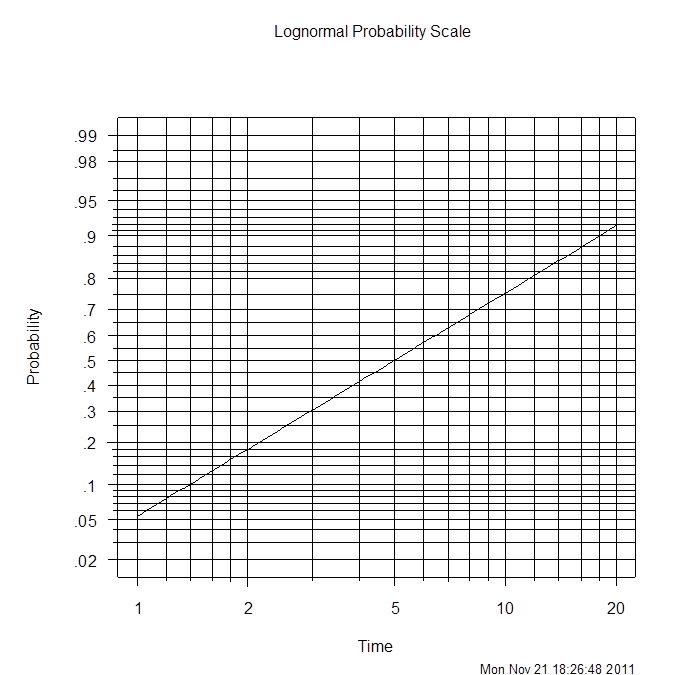
\includegraphics[width = 5in]{lognormal_graph_1.png}
  \caption{Lognormal Probability Plot}
\end{figure}

\subsection{} 
Plot on the paper the LOGNOR\begin{math}(exp(\mu) = 5, \sigma = 1).\end{math}
Explain clearly the process to plot the line.\\

A probability plot linearizes t, some variable, against the CDF of that variable by transforming both variables such that the relationship between the two is linear.  First we start with the quantile function of the CDF.  In the case of the lognormal, this is \(t_p = exp(\mu + \phi_{nor}^{-1} \sigma)\), where \(\phi_{nor}^{-1}\) is the p quantile of the standard normal distribution.  By taking the log of both sides we get \(log(t_p) = \mu + \phi_{nor}^{-1} \sigma\).  This relationship plots as a straight line.  The slope of the line, given that the respective quantile function is the inverse of  \(\phi_{nor}\) is \(1/\sigma\).\\

Therefore the steps use to generate the plot above are as follows:\\
\begin{enumerate}
\item Create a sequence of numbers between 0 and 20.\\

\item Log these numbers and calculate respective PDF outputs for the vector based on the normal distribution.  Since the numbers have been logged this is the equivalent to the lognormal distribution.

\item Use the plotprob function in Rsplida, which creates probability paper by plotting each respective axis in log-scale (in this case).

\item Use the lines() function in Rsplida which plots t:time against y:quantiles of time.
\end{enumerate}


% Problem 1.b
\begin{figure}
  \centering
  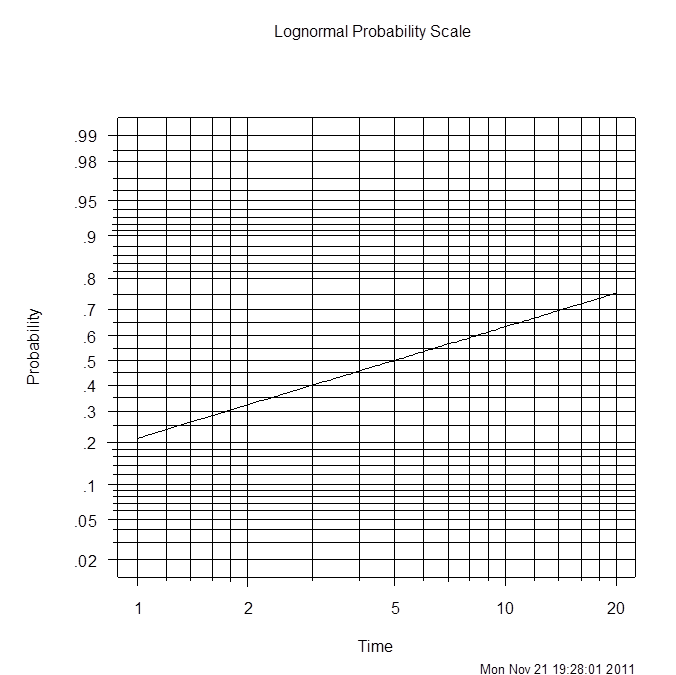
\includegraphics[width = 5in]{lognormal_graph_2.png}
  \caption{Lognormal Probability Plot}
\end{figure}
\FloatBarrier

\subsection{}
Plot on the paper the LOGNOR\begin{math}(exp(\mu) = 5, \sigma = 2).\end{math}
Explain clearly the process to plot the line.\\

A probability plot linearizes t, some variable, against the CDF of that variable by transforming both variables such that the relationship between the two is linear.  First we start with the quantile function of the CDF.  In the case of the lognormal, this is \(t_p = exp(\mu + \phi_{nor}^{-1} \sigma)\), where \(\phi_{nor}^{-1}\) is the p quantile of the standard normal distribution.  By taking the log of both sides we get \(log(t_p) = \mu + \phi_{nor}^{-1} \sigma\).  This relationship plots as a straight line.  The slope of the line, given that the respective quantile function is the inverse of  \(\phi_{nor}\) is \(1/\sigma\).\\

Therefore the steps use to generate the plot above are as follows:\\
\begin{enumerate}
\item Create a sequence of numbers between 0 and 20.\\

\item Log these numbers and calculate respective PDF outputs for the vector based on the normal distribution.  Since the numbers have been logged this is the equivalent to the lognormal distribution.

\item Use the plotprob function in Rsplida, which creates probability paper by plotting each respective axis in log-scale (in this case).

\item Use the lines() function in Rsplida which plots t:time against y:quantiles of time.
\end{enumerate}
\newpage


\section{(15 points).}
Consider the probability paper given in Figure 1. Do the following:\\

% Problem 2.a
\FloatBarrier
\begin{figure}
  \centering
  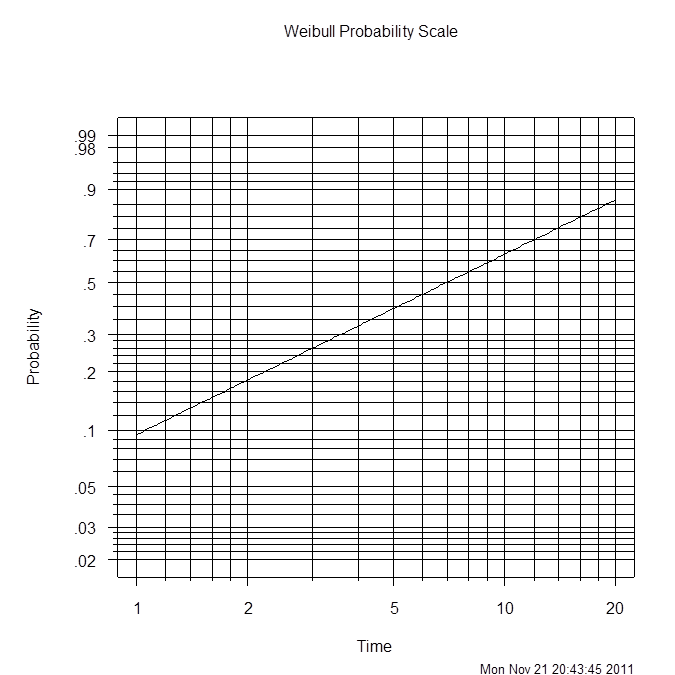
\includegraphics[width = 5in]{weibull_graph_1.png}
  \caption{Weibull Probability Plot}
\end{figure}
\FloatBarrier

\subsection{}
Plot on the paper the WEIB\begin{math}(exp(\eta = 10, \beta = 2).\end{math}
Explain clearly the process to plot the line.\\

A probability plot linearizes t, some variable, against the CDF of that variable by transforming both variables such that the relationship between the two is linear.  First we start with the quantile function of the CDF.  In the case of the Weibull, this is \(t_p = exp(\mu + \phi_{sev}^{-1} \sigma)\), where \(\phi_{sev}^{-1}\) is the p quantile of the standard smallest extreme value distribution.  By taking the log of both sides we get \(log(t_p) = \mu + \phi_{sev}^{-1} \sigma\).  This relationship plots as a straight line.  The slope of the line, given that the respective quantile function is the inverse of  \(\phi_{sev}\) is \(1/\sigma\).\\

Therefore the steps use to generate the plot above are as follows:\\
\begin{enumerate}
\item Create a sequence of numbers between 0 and 20.\\

\item Log these numbers and calculate respective PDF outputs for the vector based on the smallest extreme value distribution.  Since the numbers have been logged this is the equivalent to the Weibull distribution.

\item Use the plotprob function in Rsplida, which creates probability paper by plotting each respective axis in log-scale (in this case).

\item Use the lines() function in Rsplida which plots t:time against y:quantiles of time.
\end{enumerate}


% Problem 2.b
\FloatBarrier
\begin{figure}
  \centering
  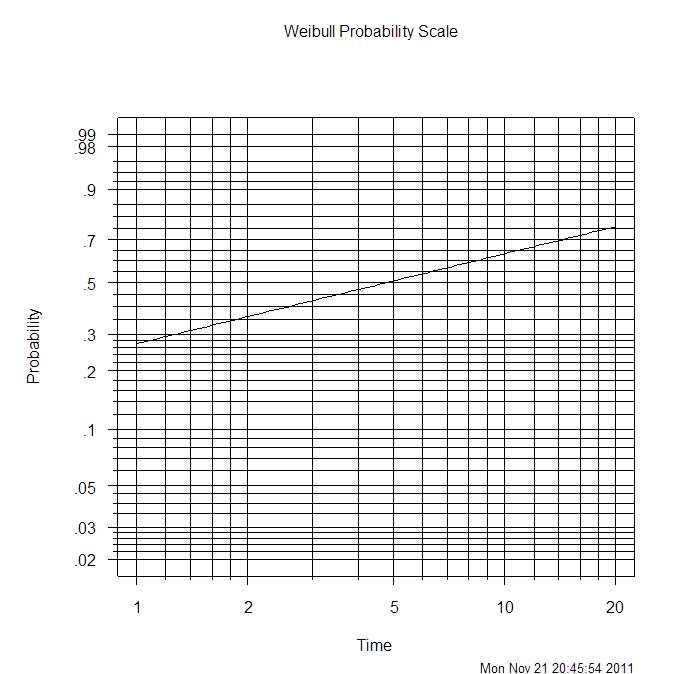
\includegraphics[width = 5in]{weibull_graph_2.png}
  \caption{Weibull Probability Plot}
\end{figure}
\FloatBarrier

\subsection{}
Plot on the paper the WEIB\begin{math}(exp(\eta = 10, \beta = 2).\end{math}
Explain clearly the process to plot the line.\\

A probability plot linearizes t, some variable, against the CDF of that variable by transforming both variables such that the relationship between the two is linear.  First we start with the quantile function of the CDF.  In the case of the Weibull, this is \(t_p = exp(\mu + \phi_{sev}^{-1} \sigma)\), where \(\phi_{sev}^{-1}\) is the p quantile of the standard smallest extreme value distribution.  By taking the log of both sides we get \(log(t_p) = \mu + \phi_{sev}^{-1} \sigma\).  This relationship plots as a straight line.  The slope of the line, given that the respective quantile function is the inverse of  \(\phi_{sev}\) is \(1/\sigma\).\\

Therefore the steps use to generate the plot above are as follows:\\
\begin{enumerate}
\item Create a sequence of numbers between 0 and 20.\\

\item Log these numbers and calculate respective PDF outputs for the vector based on the smallest extreme value distribution.  Since the numbers have been logged this is the equivalent to the Weibull distribution.

\item Use the plotprob function in Rsplida, which creates probability paper by plotting each respective axis in log-scale (in this case).

\item Use the lines() function in Rsplida which plots t:time against y:quantiles of time.
\end{enumerate}

\vspace{2cm}
\section{(20 points).}
Consider a data set with two observations.\\

\begin{center}
\begin{tabular}{c c}
\hline
Time & Status\\
\hline
1 & Fail\\
2 & Censored\\
\hline
\end{tabular}
\end{center}

\begin{enumerate}
  \begin{enumerate}
    \item Write the likelihood of the data for a lognormal model.


The likelihood is as follows:\\

\begin{math}(L(\mu, \sigma) = \prod_{i=1}^{2}\left\{\Phi_{nor}\Bigg[\frac{log(t_i) - \mu}{\sigma}\Bigg]\right\}^{\delta_{i}} \mult \left\{1- \Phi_{nor}\Bigg[\frac{log(t_i) - \mu}{\sigma}\Bigg]\right\}^{1-\delta_{i} \end{math}\\

where \(\delta_{i}\) takes the value of 1 where an obsevation is left-censored, and 0 where an observation is right-censored.

\newpage
    \item Write the likelihood of the data for a Weibull model.


The likelihood is as follows:\\

\begin{math}(L(\mu, \sigma) = \prod_{i=1}^{2}\left\{\Phi_{sev}\Bigg[\frac{log(t_i) - \mu}{\sigma}\Bigg]\right\}^{\delta_{i}} \mult \left\{1- \Phi_{sev}\Bigg[\frac{log(t_i) - \mu}{\sigma}\Bigg]\right\}^{1-\delta_{i} \end{math}\\

where \(\delta_{i}\) takes the value of 1 where an obsevation is left-censored, and 0 where an observation is right-censored.

\item Use JMP to fit the data. Provide parameter estimates and a plot of the likelihood contour surface.

\FloatBarrier
\begin{figure}
  \centering
  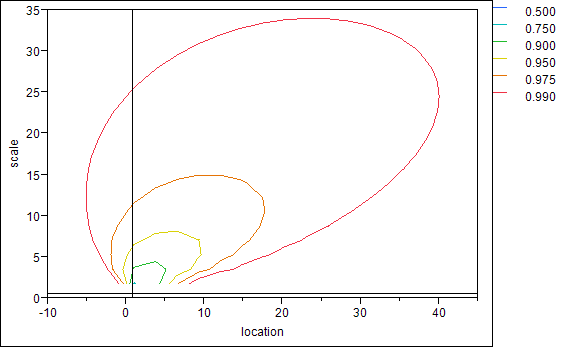
\includegraphics[width = 5in]{likelihood_fit_1.png}
  \caption{Weibull Likelihood Contour Surface}
\end{figure}
\FloatBarrier

  \end{enumerate}
\end{enumerate}


\section{(30 points).}
A component has two independent failure modes, say Mode 1 and Mode 2, respectively.  The independent failure modes can be modeled using the Weibull distributions WEIB\((\eta_{1}, \beta_{1})\) and WEIB\((\eta_{2}, \beta_{2})\), respectively.\\

Define by T the life of the component when the two failure modes are active.  From a set of failure time data, the following estimates were obtained from JMP.\\

\begin{center}
\(\hat{\eta_{1}} = 30 , \hat{\beta_{1}} = 1 \)\\
\(\hat{\eta_{1}} = 40 , \hat{\beta_{1}} = 2 \)\\
\end{center}

Using the estimates above, do the following:

\begin{enumerate}
  \begin{enumerate}
  \item Provide an estimate of the survival function \(S_T(t)\) of the component.\\
    \begin{center}
      \(\hat{S_T}(t) = \left\{1 - \hat{F_1}(t)\right\}\left\{1 - \hat{F_2}(t)\right\} \)\\
        
        where \(\hat{F_1} \) is WEIB(30, 1) and \(\hat{F_2} \) is WEIB(40, 2)\\
    \end{center}
    \vspace{0.5cm}
  \item Provide an estimate of the cdf \(F_T(t)\) of the component.\\
    \begin{center}
      \(\hat{F_T}(t) = \left\{1 - \left\{1 - \hat{F_1}(t)\right\}\left\{1 - \hat{F_2}(t)\right\}\right\} \)\\
      
      where \(\hat{F_1} \) is WEIB(30, 1) and \(\hat{F_2} \) is WEIB(40, 2)\\
    \end{center}
\pagebreak
  \item Obtain an expression for the hazard estimate of \(T \). Your answer must be in function of hazard functions (\ h_1(t) \) and \(h_2(t) \) for failures from Mode 1 and Mode 2, respectively.\\

  \begin{center}
    \large\(h(t) = \frac{f(t)}{1 - F(t)}\)\\
      \vspace{1cm}
    \(\frac{f_1(t)f_2(t)}{1-\left\{1 - [1 - F_1(t)][1 - F_2(t)]\right\}} \)\\
      \vspace{1cm}
    \(\frac{f_1(t)f_2(t)}{[1 - F_1(t)][1 - F_2(t)]} = h_1(t)h_2(t) \)\\
  \end{center}

\vspace{3in}
  \item Plot the hazard function of \(T \). Make relevant comments.\\

  \begin{center}
        \FloatBarrier
      \begin{figure}
        \centering
        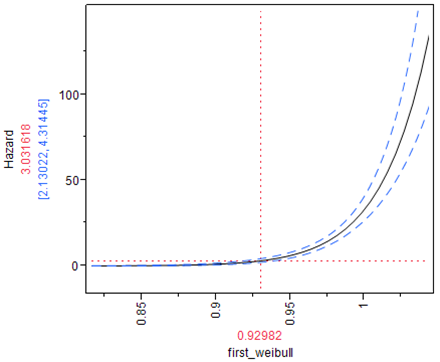
\includegraphics[width = 5in]{prob4d_weibull_1_haz.png}
        \caption{Hazard of \(T \) distributed \( WEI(\eta = 30 , \beta = 1)\)}
      \end{figure}
      \FloatBarrier
  \end{center}
  
   \begin{center}
        \FloatBarrier
      \begin{figure}
        \centering
        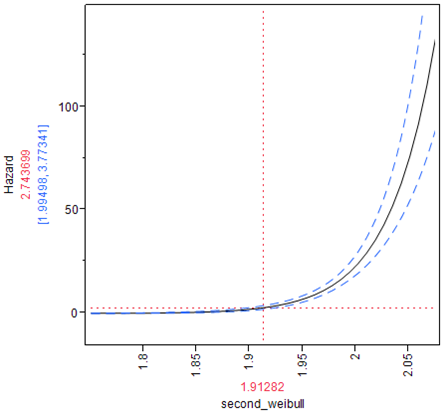
\includegraphics[width = 5in]{prob4d_weibull_2_haz.png}
        \caption{Hazard of \(T \) distributed \( WEI(\eta = 30 , \beta = 1)\)}
      \end{figure}
      \FloatBarrier
  \end{center}
  
   \begin{center}
        \FloatBarrier
      \begin{figure}
        \centering
        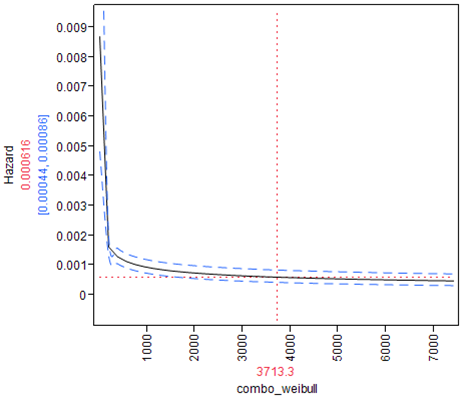
\includegraphics[width = 5in]{prob4d_weibull_combo_haz.png}
        \caption{Hazard of \(T \) distributed \( WEI(\eta = 30 , \beta = 1)\)}
      \end{figure}
      \FloatBarrier
  \end{center} 
  
  \end{enumerate}
\end{enumerate}

\section{} Use the ShockAbsorber data with failure modes to work on this question.

\begin{enumerate}
  \begin{enumerate}
  \item Fit the data without using the information on failure modes.\\

\begin{center}
        \FloatBarrier
      \begin{figure}
        \centering
        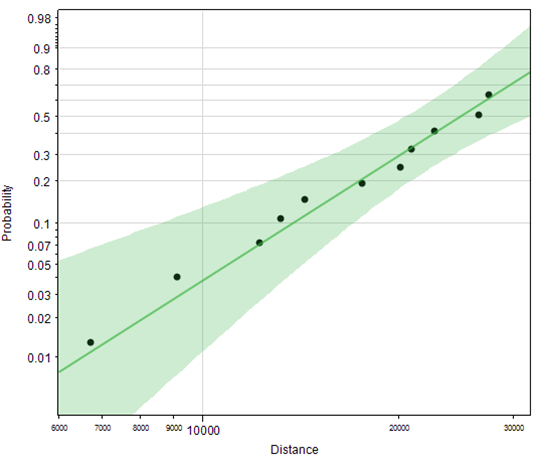
\includegraphics[width = 5in]{problem5_fit.png}
        \caption{CDF of the Weibull model without respect to failure mode.}
      \end{figure}
      \FloatBarrier
  \end{center}
  
  \item Use a Weibull for the two modes of failure and the information on failure mode to estimate failure time when the two moes of failure are acting.\\

\begin{center}
        \FloatBarrier
      \begin{figure}
        \centering
        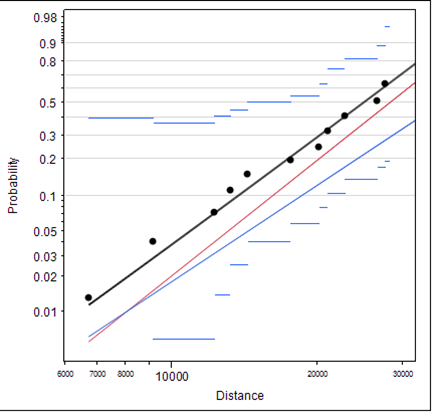
\includegraphics[width = 5in]{problem5_fit_twomodes.png}
        \caption{CDF of the Weibull model with respect to failure mode.}
      \end{figure}
      \FloatBarrier
  \end{center}
  
  \item Compre the two models fitted above. Explain throughly differences or similarities you observe in the two model fits. For this, it would be convenient to provide graphical comparisons for the failure probabilities and hazard function estimates from the two models.
  
  \begin{center}
        \FloatBarrier
      \begin{figure}
        \centering
        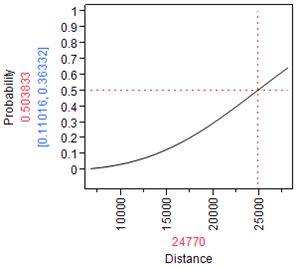
\includegraphics[width = 5in]{problem5_fit_dist1.png}
        \caption{CDF of the first model (wo failure modes)}
      \end{figure}
      \FloatBarrier
  \end{center}
  
  \begin{center}
        \FloatBarrier
      \begin{figure}
        \centering
        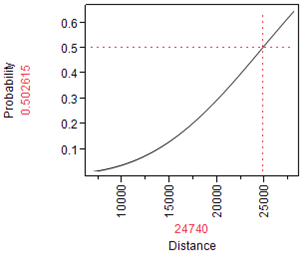
\includegraphics[width = 5in]{problem5_fit_dist2.png}
        \caption{CDF of the second model (w failure modes)}
      \end{figure}
      \FloatBarrier
  \end{center}
 
  Modeling for failure modes does not appear to add much information to the understanding of the data generating process.  The mean time to failure of both models is about 24,700 thousand cycles each.
  
\begin{center}
First Model\\
\begin{tabular}{c c c}
\hline
Parameter & Estimate & Std Error\\
\hline
Weibull \(\alpha \) & 27718 & 3046\\
Weibull \(\beta \) & 3.16 & 0.73\\
\hline
\end{tabular}
\end{center}

\begin{center}
Second Model\\
\begin{tabular}{c c}
\hline
Parameter & Estimate\\
\hline
Weibull - Mode 1 \(\alpha \) & 31205\\
Weibull - Mode 1 \(\beta \) & 3.38\\
Weibull - Mode 2 \(\alpha \) & 40865\\
Weibull - Mode 2 \(\beta \) & 2.82\\
\hline
\end{tabular}
\end{center}
  
Further, the hazard estimates at 20,000 thousand cycles for both models is very close, about 0.00005.\\

\begin{center}
        \FloatBarrier
      \begin{figure}
        \centering
        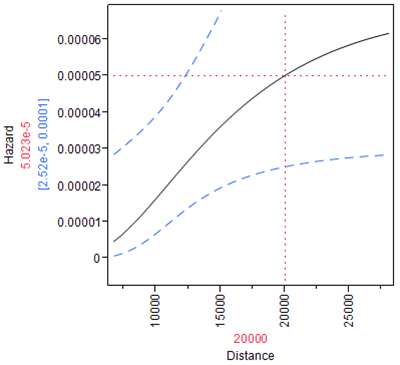
\includegraphics[width = 5in]{problem5_hazard1.png}
        \caption{Hazard of the Weibull model without respect to failure mode.}
      \end{figure}
      \FloatBarrier
  \end{center}
  
  \begin{center}
        \FloatBarrier
      \begin{figure}
        \centering
        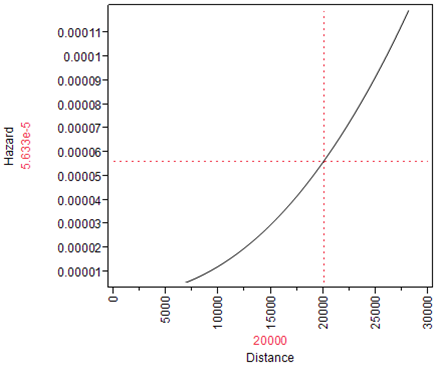
\includegraphics[width = 5in]{problem5_hazard2.png}
        \caption{Hazard of the Weibull model with respect to failure mode.}
      \end{figure}
      \FloatBarrier
  \end{center}\\

    \end{enumerate}
\end{enumerate}

\end{document}
